\chapter{Training Private Models That Know What They Don't Know}

\section{Additional Method Details}

\subsection{DP-SGD Algorithm}

We provide a detailed definition of DP-SGD in Algorithm~\ref{alg:dpsgd}.

	\vspace{10pt}
    \begin{algorithm}[H]
	\caption{DP-SGD~\citep{abadi2016deep}}\label{alg:dpsgd}
	\begin{algorithmic}[1]
	\Require Training dataset $D$, loss function $\ell$, learning rate $\eta$, noise multiplier $\sigma$, sampling rate $q$, clipping norm $c$, iterations $T$.
		\State {\bf Initialize} $\theta_0$
		\For{$t \in [T]$}
		\State {\bf 1. Per-Sample Gradient Computation}
		\State Sample $B_t$ with per-point prob. $q$ from $D$
		\For{$i \in B_t$}  
		\State $g_t(\bm{x}_i) \gets \nabla_{\theta_t} \ell(\theta_t, \bm{x}_i)$
		\EndFor
		\State {\bf 2. Gradient Clipping}
		\State {$\bar{g}_t(\bm{x}_i) \gets g_t(\bm{x}_i) / \max\big(1, \frac{\|g_t(\bm{x}_i)\|_2}{c}\big)$}\label{alg:dpsgd_clipping}
		\State {\bf 3. Noise Addition}
		\State {$\tilde{g}_t \gets \frac{1}{|B_t|}\left( \sum_i \bar{g}_t(\bm{x}_i) + \mathcal{N}(0, (\sigma c)^2 \mathbf{I})\right)$}\label{alg:dpsgd_noise}
		\State { $\theta_{t+1} \gets \theta_{t} - \eta \tilde{g}_t$}
		\EndFor
		\State {\bf Output} $\theta_T$, privacy cost $(\varepsilon, \delta)$ computed via a privacy accounting procedure
	\end{algorithmic}
\end{algorithm}

\section{Additional Experimental Details}

\subsection{Hyperparameters}
\label{sec:hyp}

In this section, we document additional hyper-parameter choices. For Self-Adaptive Training (\sat), we set the pre-training epochs to $100$ and momentum parameter $0.9$. For Selective Classification Training Dynamics (\sctd), we set the weighting parameter $k=3$ and consider checkpoints at a $50$ batch resolution. For Monte-Carlo Dropout, we set the dropout probability to $0.1$. Entropy regularization as suggested in~\citet{feng2023towards} is employed with $\beta = 0.01$.

\subsection{Class Imbalance Experiments}
\label{sec:class_imb_real}

We provide additional experiments on the effect of class imbalance to extend our intuition from Section~\ref{sec:dp_affects_sc}. To that end, we take two data sets from our main results, namely CIFAR-10 and FashionMNIST, and produce four alternate datasets from each dataset. These datasets feature various degrees of class imbalance with $p_0 \in \{0.5,0.25,0.1,0.01\}$ specifying the sampling probability for class $0$. All other classes maintain a sampling probability of $1$. We then train the same model as described in Section~\ref{sec:exp} and apply the softmax response SC algorithm. 

We document these results in Figures~\ref{fig:cifar10_classimb} and \ref{fig:fashionmnist_classimb}. For $\varepsilon = \infty$, we observe the expected gains from SC: minority points are accepted towards the end of the coverage spectrum~\citep{jones2020selective} and correct points are accepted first. This effect is independent of the sampling probability $p_0$. As we decrease the $\varepsilon$ budget we observe that (i) the acceptance of minority groups starts to spread over the full coverage spectrum; (ii) the accuracy on the subgroup increasingly deteriorates with smaller $\varepsilon$, and (iii)~wrongful overconfidence on the minority reverses the acceptance order at low sampling probabilities~$p_0$ (\ie incorrect points are often accepted first). These results indicate that employing selective classification on private data can have unwanted negative effects in the presence of subgroups. Future work should investigate this connection more thoroughly.

\begin{figure*}[t]
  \centering
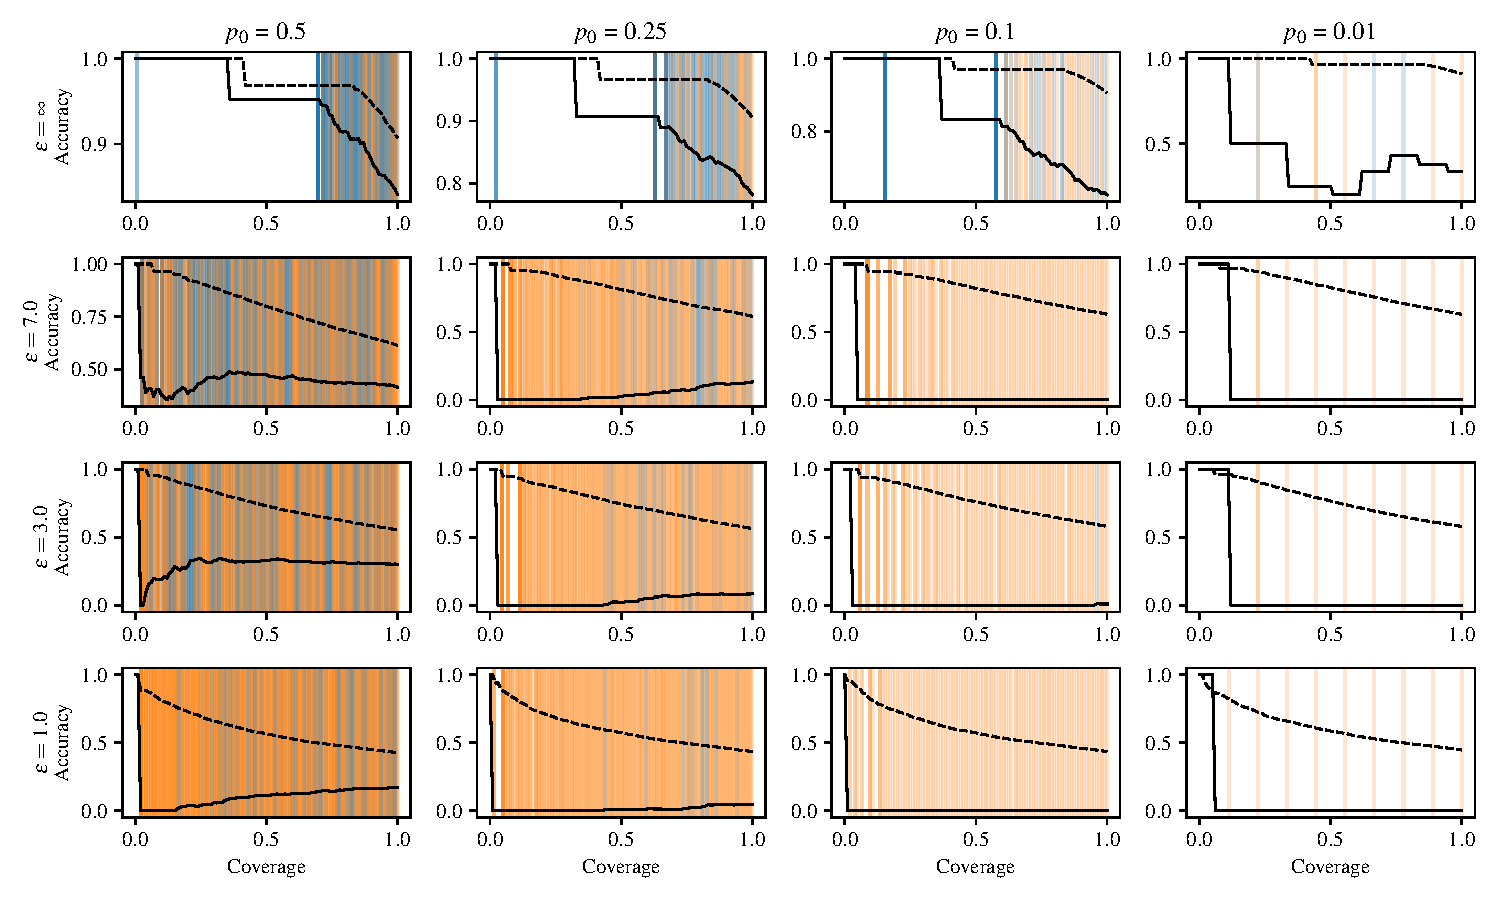
\includegraphics[width=\linewidth]{figs/sptd_dp/cifar10_classimb.pdf}
\caption[Inducing a class imbalance on CIFAR-10]{\textbf{Inducing a class imbalance on CIFAR-10}. We train multiple CIFAR-10 models across privacy levels and sampling probabilities for class 0 given by $p_0$. We plot the accuracy/coverage trade-off as well at the exact coverage level at which any point from the minority class is accepted. The accuracy-coverage trade-off for the full dataset is given by the dashed line while the trade-off for the minority group only is given by the solid line. Blue vertical lines show correctly classified points, orange points show incorrectly classified points. Non-private models accept correct points first and do so at the end of the coverage spectrum (\ie majority points are accepted first). As we increase privacy (\ie decrease $\varepsilon$), the model is increasingly unable to rank minority examples based on prediction correctness and even accepts incorrect points first. Moreover, the accuracy of the model on the minority class decreases with stronger DP. These effects are especially strong for small sampling probabilities.}
\label{fig:cifar10_classimb}
\end{figure*}

\begin{figure*}[t]
  \centering
	  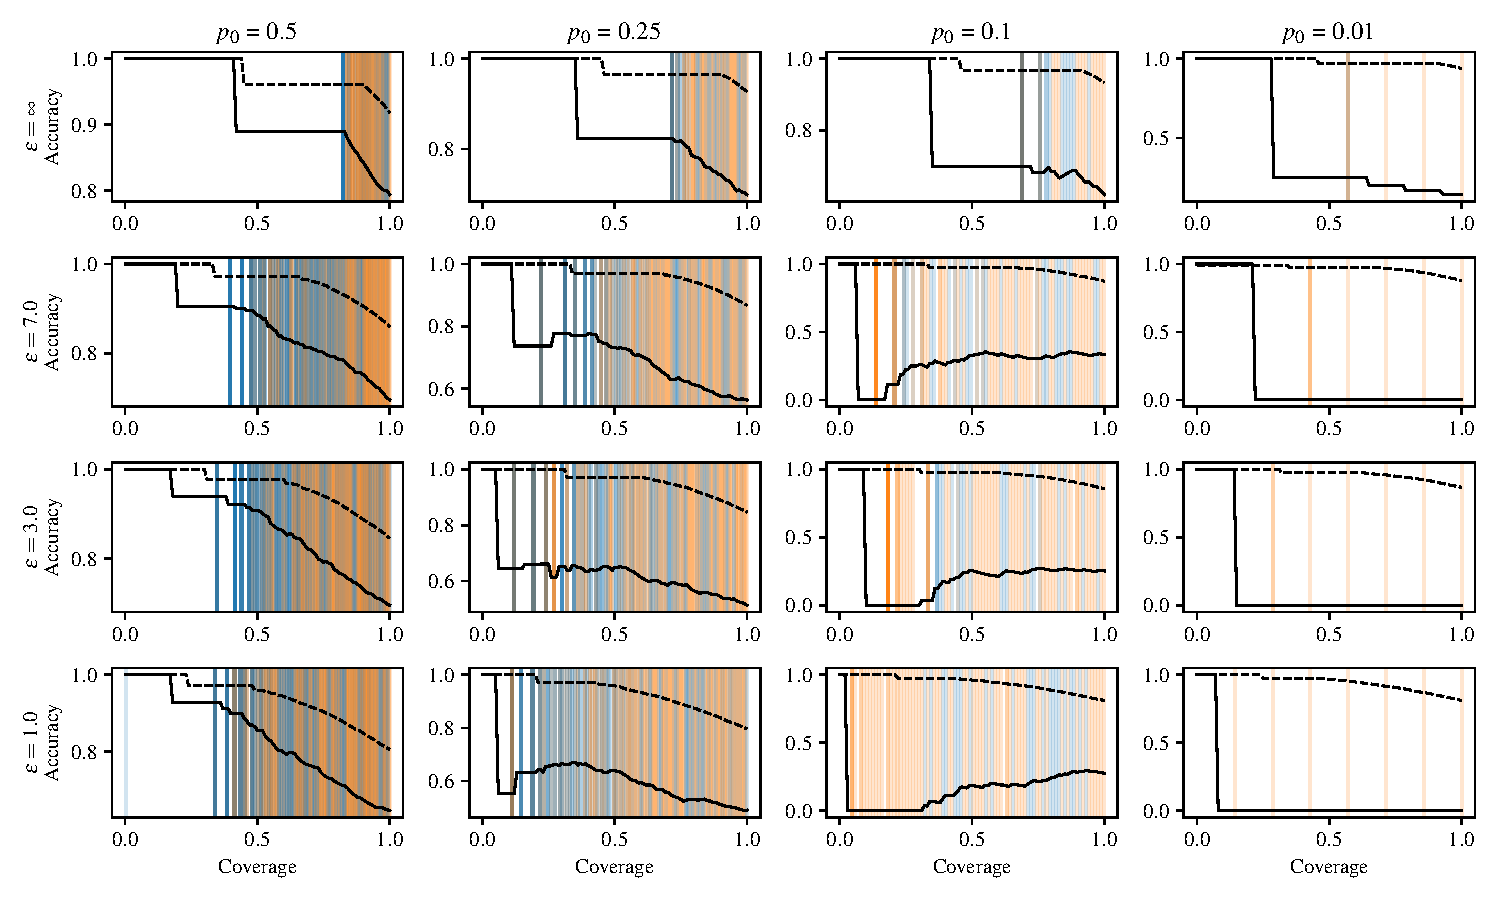
\includegraphics[width=\linewidth]{figs/sptd_dp/fashionmnist_classimb.pdf}
  
\caption[Inducing a class imbalance on FashionMNIST.]{\textbf{Inducing a class imbalance on FashionMNIST}. Same insights as in Figure~\ref{fig:fashionmnist_classimb}.}
\label{fig:fashionmnist_classimb}
\end{figure*}

\subsection{Upper Bound Reachability}
\label{sec:opt_bound_reach}

In Equation~\ref{eq:bound}, we have introduced an upper bound on the selective classification performance on a model with full-coverage accuracy $a_\text{full}$. We now present a simple experimental panel across varying full-coverage accuracy levels showing that this bound is in fact reachable by a perfect selective classifier.

We assume a binary classification setting for which we generate a true label vector $\bm{y} \in \{0,1\}^{n_0 + n_1}$ with balanced classes, \ie $n_0 = n_1$ where $n_0$ corresponds to the number points labeled as $0$ and $n_1$ corresponds to the number points labeled as $1$. Then, based on a desired accuracy level $a_\text{full}$, we generate a prediction vector $\bm{p}$ which overlaps with $\bm{y}$ for a fraction of $a_\text{full}$. Finally, we sample a  scoring vector $\bm{s}$ where each correct prediction is assigned a score $s_i \sim \mathcal{U}_{0,0.5}$ and each incorrect prediction is assigned a score $s_i \sim \mathcal{U}_{0.5,1}$. Here, $\mathcal{U}_{a,b}$ corresponds to the uniform distribution on the interval $[a,b)$. This score is clearly optimal since thresholding the scoring vector $\bm{s}$ at $0.5$ perfectly captures correct/incorrect predictions: all $s_i < 0.5$ correspond to a correct prediction, while all $s_i \geq 0.5$ correspond to an incorrect prediction. Computing the accuracy/coverage trade-off of this experiment, across various utility levels, matches the bound exactly. 

\begin{figure*}[t]
  \centering
	    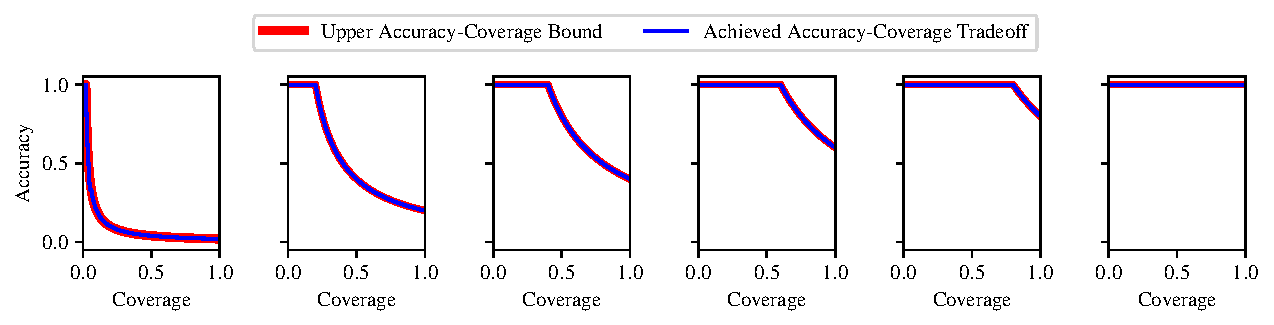
\includegraphics[width=\linewidth]{figs/sptd_dp/bound_reachability.pdf}

\caption[Upper bound matching experiment.]{\textbf{Upper bound matching experiment}. The experiment as described in Section~\ref{sec:opt_bound_reach} matches the optimal bound exactly across multiple full-coverage accuracy levels.}
\label{fig:bound_reachability}
\end{figure*}